%%% template.tex
%%%
%%% This LaTeX source document can be used as the basis for your technical
%%% paper or abstract. Intentionally stripped of annotation, the parameters
%%% and commands should be adjusted for your particular paper - title, 
%%% author, article DOI, etc.
%%% The accompanying ``template.annotated.tex'' provides copious annotation
%%% for the commands and parameters found in the source document. (The code
%%% is identical in ``template.tex'' and ``template.annotated.tex.'')

\documentclass[conference]{acmsiggraph}

\TOGonlineid{45678}
\TOGvolume{0}
\TOGnumber{0}
\TOGarticleDOI{1111111.2222222}
\TOGprojectURL{}
\TOGvideoURL{}
\TOGdataURL{}
\TOGcodeURL{}

\title{The Title of Your Paper Goes Here}

\author{Yanling He\thanks{e-mail:heyl@cs.washington.edu}\\Computer Science \& Engineering\\University of Washington
\and
Xin Yang\thanks{e-mail:yx1992@cs.washington.edu}\\Computer Science \& Engineering\\University of Washington
\and
Xiaoyi Zhang\thanks{e-mail:xiaoyiz@cs.washington.edu}\\Computer Science \& Engineering\\University of Washington
}
\pdfauthor{Yanling He}
\pdfauthor{Xin Yang}
\pdfauthor{Xiaoyi Zhang}

\keywords{data visualization, instagram, filter, hashtag}

\begin{document}

%% \teaser{
%%   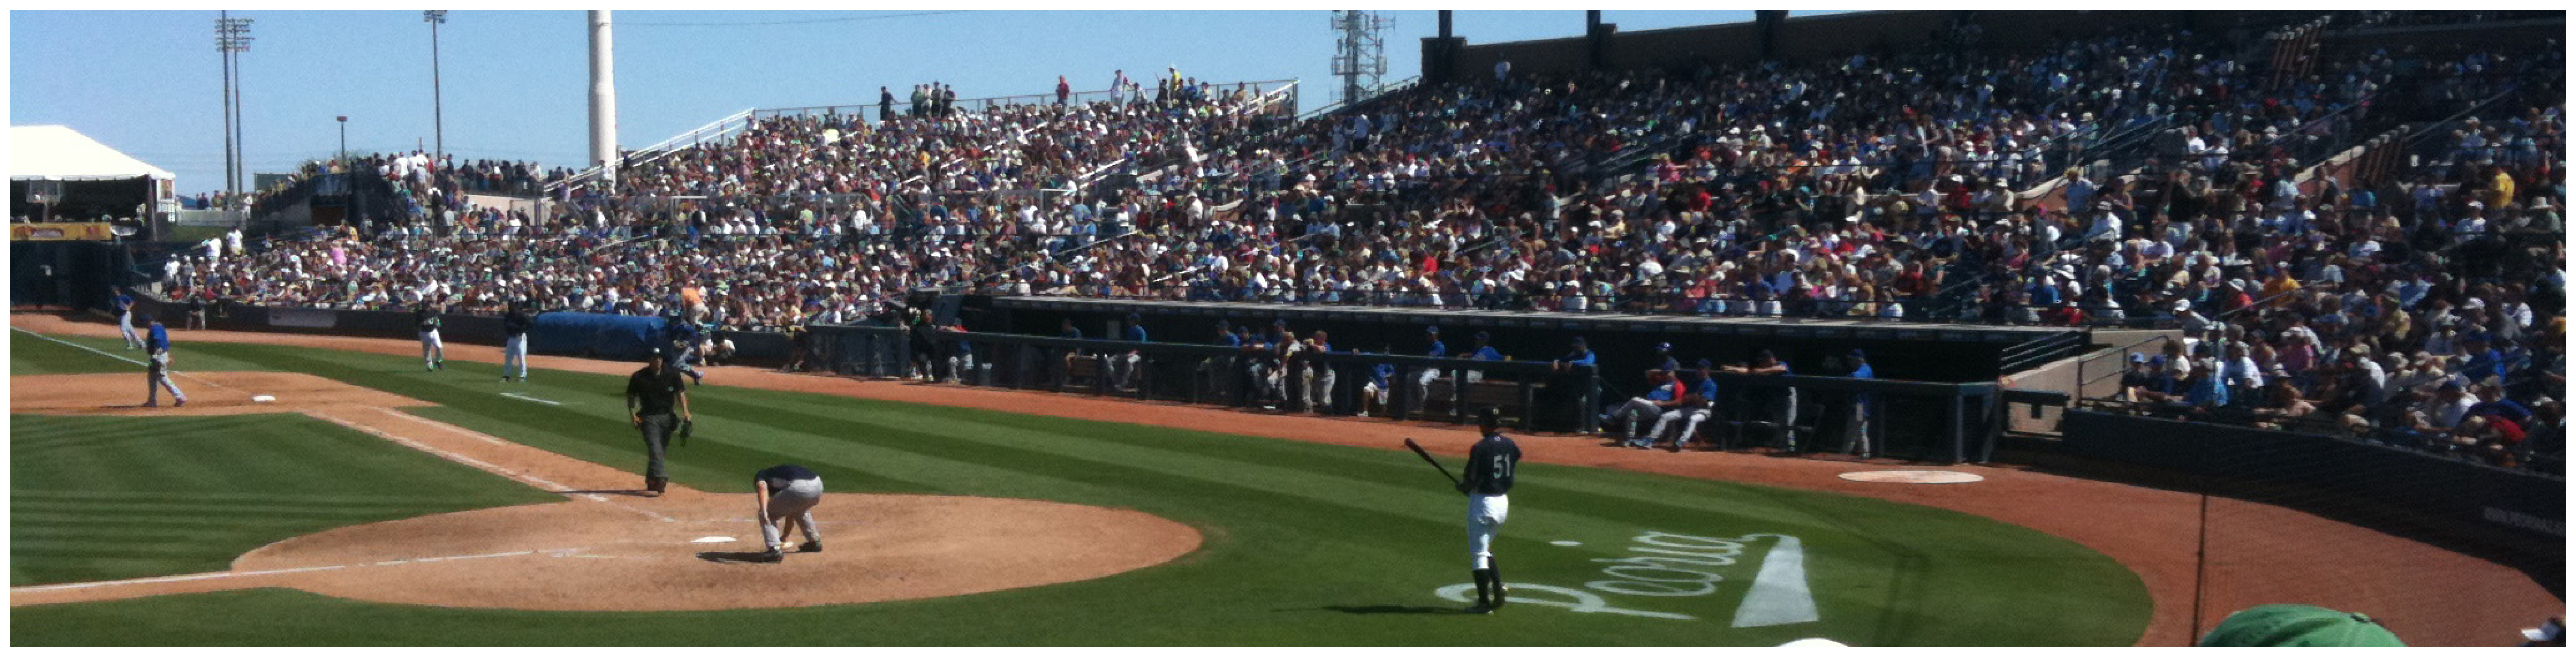
\includegraphics[height=1.5in]{images/sampleteaser}
%%   \caption{Spring Training 2009, Peoria, AZ.}
%% }

\maketitle

\begin{abstract}

Because of the spread of the Internet, social platforms bacome big data pools. From there we can learn about the trends, culture and hot topics.  This project focuses on analyzing the data from Instagram. It shows the relationship of Instagram filter data with location and number of likes to give users filter suggestion on achieving more likes based on their location. It also analyzes the popular hashtags in different locations to show visual culture differences between different cities. 

\end{abstract}

\keywordlist

%% Use this only if you're preparing a technical paper to be published in the 
%% ACM 'Transactions on Graphics' journal.

\TOGlinkslist

%% Required for all content. 

\copyrightspace

\section{Introduction}

As "a picture is worth a thousand words", more and more people are sharing their daily life, personal interests, news and events using images on social platform. Instagram is such a platform which is a popular mobile photo sharing application. It launched in October 2010, and rapidly gained popularity, with over 100 million active users as of April 2012 and over 300 million as of December 2014. Because of these huge amount of information in the dataset of Instagram, and we are interested in analyzing and visualizing the patterns of them. 

This project is focusing on analyzing Instagram data to learn about the culture differences between different places. This project analyzes how filter usage are distributed in 50 cities, which are the cities with most population in each state of United States. This give us the information about how filter preference and vision culture varies in different states. The project also analyzes the number of hashtags been labeled on the posts for each city. It shows the popular hashtags for each city which reveal the popular event or hot terms in different cities.

While you are using the Instagram, you may also have ever scrolled through the Instagram filter list back and force worrying about which one to use, and how to make more people like it. But since culture background and contents varies a lot from photo to photo, it is hard to make a simple suggestion that let everyone like it. Our project also analyzes the Instagram filter data based on location and like to help you solve this problem.

The goal of this project is to learn about visual culture and content differences to help catch both the artistic trends and event trends for different places. It can also help user to make better filter selection to improve photo quality and reach more likes.   

\section{Related Work}

Due to the popularity and the amount of data information, there are couple groups of people are also interested in the culture information reflected in the Instagram photo data. Hochman's Zooming into an Instagram city \cite{hochman13} \cite{hochman12} visualizes and analyzes samples from a data set of about 550,000 Instagram photos from New York City and Tokyo, by applying visualization and Cultural Analytics techniques. They show all the images in the collection. They download data based on latitude and longitude criteria and use specified tools to analyze the data. One interesting result of this paper is that there seem to be reoccurring spatio-temporal visual deviations in a specific time period and a set place. Based on those large sets of Instagram photos, they show how visual social media can be analyzed at multiple spatial and temporal scales. They also present analysis of social and cultural dynamics in specific places and particular times, and introduce new visualization techniques which can show tens of thousands of individual images sorted by their metadata or algorithmically extracted visual features. But as they only focuses on photo color and photo style, but our project cares more anout the label information and filter data. They shows the differences of visual styles in different time different cities, while we are analyzing the exact events and objects that people are captured and marked in different cities.

There are also some existing analytical tools for Instagram. Iconosquare (formerly Statigram) \cite{iconosquare} provides useful statistics about Instagram. It can also respond to comments and monitor hashtags. Instagram-analytics \cite[simplymeasured] contains huge amount of raw instagram data for users. Instastats \cite{instastats} is python scripts to pull data from Instagram API. Those work shows us what data information are available from Instagram and our project uses some of the tools to get our desired data for analysis.

\section{Methods}

\subsection{Data Preparation}
\subsection{Data Preparation}

In order to find interesting pattern from the raw data, we use python script to process the data. We first explore the relationship between filter and number of likes. We ignore the location and get the whole table of filter, number of photos with this filter, maximal likes, average likes and total number of likes.  With the help of Tableau, we can see the following result in figure \ref{like-filter},\ref{normal} and \ref{no-normal}.


\begin{figure}[ht]
  \centering
  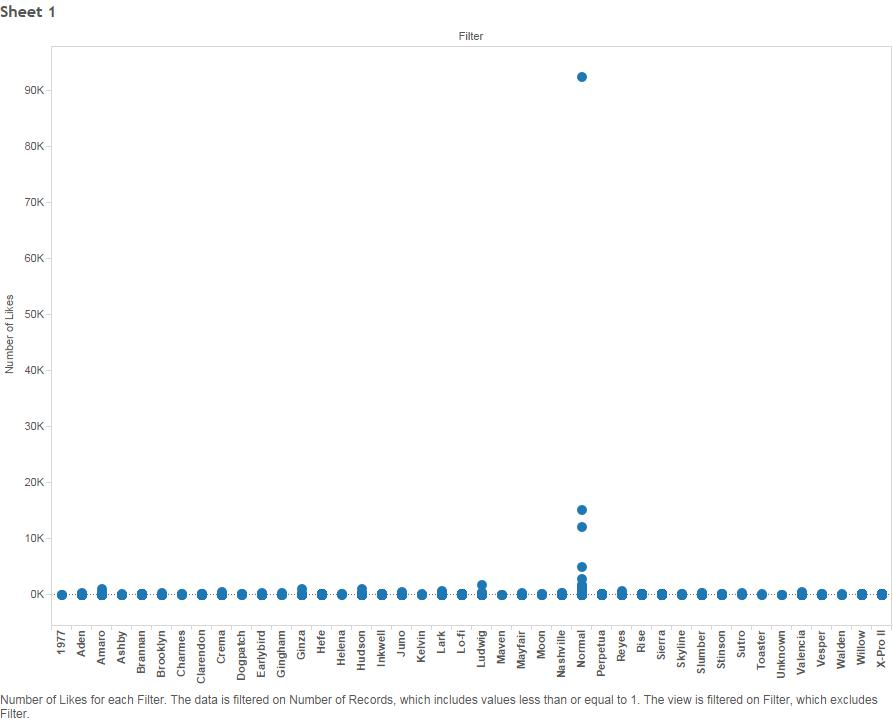
\includegraphics[width=3in]{images/sample_all_filter-like}
  \caption{Likes and filters in Seattle}
  \label{like-filter}
\end{figure}
\begin{figure}[ht]
  \centering
  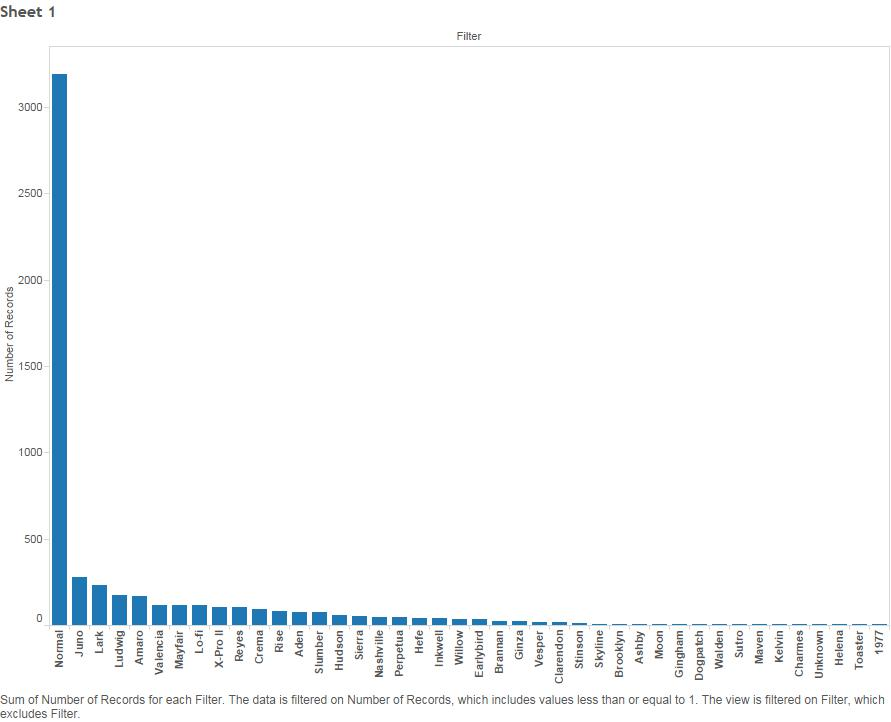
\includegraphics[width=3in]{images/sample_all_number-filter_sorted}
  \caption{Number of photos in different filters}
  \label{normal}
\end{figure}
\begin{figure}[ht]
  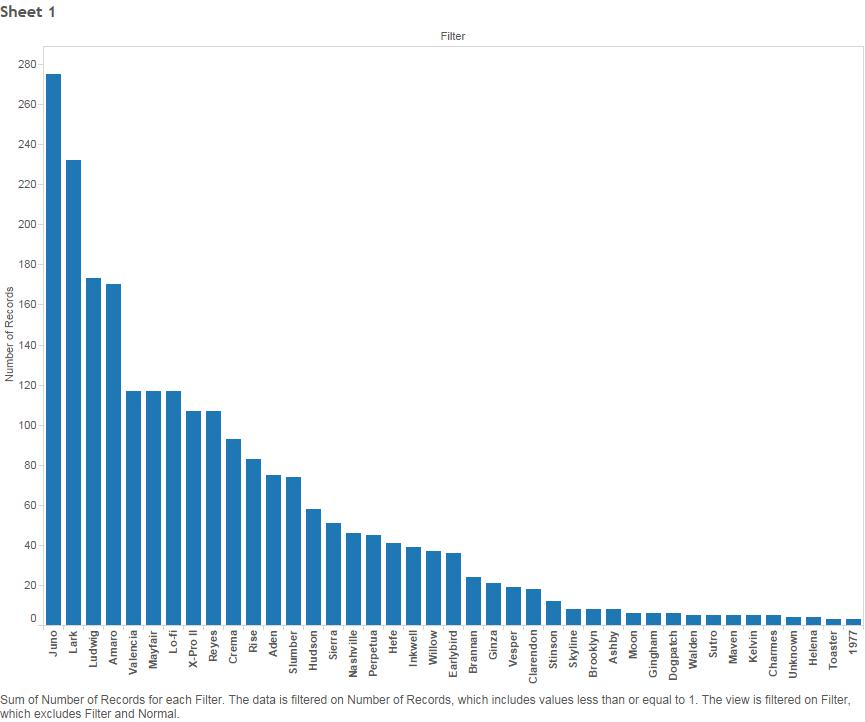
\includegraphics[width=3in]{images/sample_all_number-filter_sorted_no-normal}
  \centering
  \caption{Number of photos in different filters. Normal excluded}
  \label{no-normal}
\end{figure}



We can see that the normal filter appears dominantly. This is probably because normal filter is the default setting of Instagram. Therefore if people are not very familiar with Instagram, then they will hardly pick up advanced filters. So many filters use normal filter that most popular photos are using normal filters. If we remove the effect of normal filters, we can see that the curve of  number of photos on filters looks like an exponential function, which is an evidence that it may  follow the power law. It is reasonable, since power law is a common phenomenon in social network.
In this way, we may design a recommendation system for filters:
since normal filter is so common,
we can help users to use other advanced filters,
in this way users may obtain sense of accomplishment while achieving lots of likes.


We also study the relationship between the likes and the hashtag. We create the table of word, total like, average like and maximal like for each city. The following chart is the result for Seattle.
\begin{figure}[ht]
  \centering
  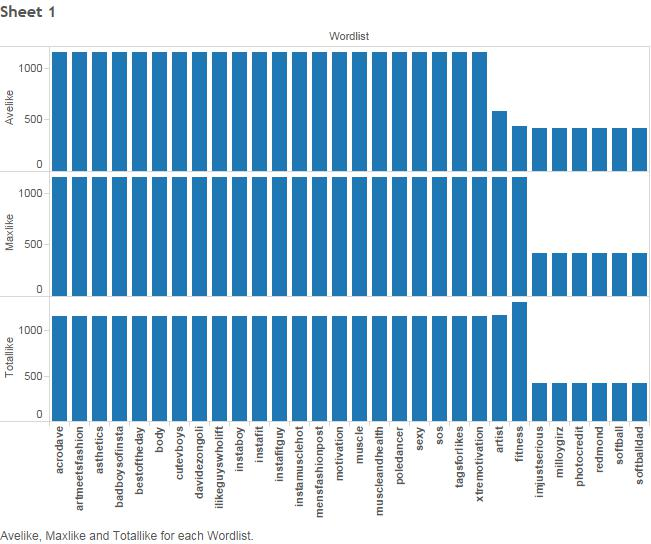
\includegraphics[width=3in]{images/sample_Seattle_like_word}
  \caption{Hot hashtags in Seattle}
\end{figure}
We do not find interesting pattern in the chart. We think the main reason is that we do not have enough data. Most hashtag appear only 1 or 2 times, which is too few to analyze. However, we can still observe that hashtags with popular photos are “meaningful”, that is , we can see some kind of trend from the hot hashtags. This can be used to notice users what is happening now in the city.



\section{Future Work}

\subsection{Computer Vision Analysis}
Since not all the photos are labeled with hashtags and not all the hashtags are correctly showing the content in each photo, using computer vision to analysis the real photo content, the style of the scenes and the major color theme may have stronger correlation with the filter types.
\subsection{Relationship with Time}
As the time changes people’s vision preference may also changes, so the preference of filters may shifts as the time changes, we can learn the relationship with filters, likes and time to learn how visual preference changes and give out more current filter suggestion.
\subsection{World Map}
Since all the location analysis are based on the United States, so culture variety may be less between each cities, to extend the data to world based to learn some culture different between continents may give us more meaningful data. But world-wise spread of the Instagram usage may be the limit of this extension.

\section{Conclusion}

Lorem ipsum dolor sit amet, consectetur adipisicing elit, sed do
eiusmod tempor incididunt ut labore et dolore magna aliqua. Ut enim ad
minim veniam, quis nostrud exercitation ullamco laboris nisi ut
aliquip ex ea commodo consequat. Duis aute irure dolor in
reprehenderit in voluptate velit esse cillum dolore eu fugiat nulla
pariatur. Excepteur sint occaecat cupidatat non proident, sunt in
culpa qui officia deserunt mollit anim id est laborum.


\begin{thebibliography}{10}

\bibliographystyle{acmsiggraph}
\bibliography{template}

\bibitem[1]{hochman13}
  [1] Hochman, Nadav \& Manovich, Lev. (2013) Zooming into an Instagram City: Reading the local through social media,
  \emph{ First Monday.}
  
\bibitem[2]{hochman12}
  [2] Hochman, Nadav \& Schwartz, Raz. (2012) Visualizing instagram: Tracing cultural visual rhythms,
  \emph{Proceedings of the Workshop on Social Media Visualization (SocMedVis) in conjunction with the Sixth International AAAI Conference on Weblogs and Social Media.}
  (ICWSM--12), (pp. 6--9).
  
\bibitem[3]{iconosquare}
  [3] http://iconosquare.com/
  
\bibitem[4]{simplymeasured}
  [4] http://simplymeasured.com/freebies/instagram-analytics
  
\bibitem[5]{instastats}
  [5] https://github.com/rldw/instastats
  
\end{thebibliography}

\end{document}
